\documentclass{article}
\usepackage[margin=1in]{geometry}
\usepackage{amsfonts, amsmath, amssymb}
\usepackage[none]{hyphenat}% prevents LaTeX from adding hyphenated words
\usepackage{fancyhdr} %helps introduce fancy headers and footers in the document
\usepackage{graphicx}
\usepackage{float}
\usepackage{setspace}
\usepackage[nottoc, notlot, notlof]{tocbibind}
\usepackage{hyperref}

\pagestyle{fancy}%notice the use of "fancy" instead of 'empty' here, as we don't want empty headers and footers. instead we want 'fancy' headers and footers
\fancyhead{}
\fancyfoot{}
\fancyhead [L]{\slshape {PH1102 Experiment - 02}}
%\fancyhead[places i.e. L for left, C for cenntre and R for right]{text} is for creating fancy headers. Similarly, \fancyfoot[places]{footer} can be used to set up fancy footers.
%\slshape is for italicising the text in {}. Functions of \MakeLowercase{}, \MakeUppercase{}, \MakeRobust{} are understood from their names !
\fancyhead[R]{{Priyanshu Mahato(\color{magenta} \href{mailto:pm21ms002@iiserkol.ac.in}{pm21ms002@iiserkol.ac.in})}}
\fancyfoot[C]{\thepage}%\thepage is for showing page numbers
%\renewcommand{\headrulewidth}{0pt} this is for reducing the width of the header line to 0, thus removing it
\renewcommand{\footrulewidth}{1pt} %there isnt a line in the footer by default. This helps create one.

\setlength{\headheight}{13.59999pt}
\setlength\parindent{0em}%to set custom paragraph indentation
%\setlength\parskip{5em}%to set custom space between simultaneous paragraphs
\renewcommand{\baselinestretch}{1.8}%to set custom spacing between lines
%\setstretch{1.8} this uses the setspace package to set custom spcing between lines

\usepackage{listings}
\usepackage{color}

\definecolor{dkgreen}{rgb}{0,0.6,0}
\definecolor{gray}{rgb}{0.5,0.5,0.5}
\definecolor{mauve}{rgb}{0.58,0,0.82}

\lstset{frame=tb,
	language=Python,
	aboveskip=3mm,
	belowskip=3mm,
	showstringspaces=false,
	columns=flexible,
	basicstyle={\small\ttfamily},
	numbers=none,
	numberstyle=\tiny\color{gray},
	keywordstyle=\color{blue},
	commentstyle=\color{dkgreen},
	stringstyle=\color{mauve},
	breaklines=true,
	breakatwhitespace=true,
	tabsize=3
}


\begin{document}
	\thispagestyle{empty}%removes page number only from that page
	\begin{titlepage}
		\begin{center}
			\vspace{1cm}
			\Large\textbf{Physics Laboratory PH1102}\\
			\vspace{1cm}
			\large\textbf{Lab Report}
			\vfill%fills rest of the page with spaces and adjusts as you add elements to the page
			\line(1,0){450}\\[16pt]%creates a line
			\huge\textbf{Experiment No.: 02}\\[10pt]
			\Large\textbf{- Verification of Newton's Second Law -}\\[15pt]
			\line(1,0){450}
			\vfill
			By : Priyanshu Mahato\\
			Roll No. : pm21ms002\\%can't use # without a \ : \#
			\today\\%for today's date	\\		
			
		\end{center}
	\end{titlepage}
	
	\tableofcontents%automatically generates table of contents
	
	\clearpage%clears rest of the text from the current page and shoves it forcibly to start from the next page
	
	\section{Aim}
	To verify Newton’s Second law of motion using Air Track method.
	
	\section{Apparatus Required}
	Tracking Camera, Air Track Setup, Slider, Air Pump (to adjust the air flow along 
	the track on which the slider moves and thus reduce friction), weights which can be 
	put on the slider and the pulley to adjust mass and force on the slider. The Videocom 
	Software interfaces between the air-track apparatus and a computer to collect and 
	analyze data.
	
	\section{Experimental Setup}
	The hanging weight is connected (by a string) to a movable setup (slider) on an almost 
	frictionless surface. The friction is minimized using an Air Track. A tracking camera is 
	also set up to record the data about the position of the slider (equipped with a 
	retroreflecting foil) at different instances of time. The schematic diagram is as below:
	
	\begin{figure}[H]
		\centering
		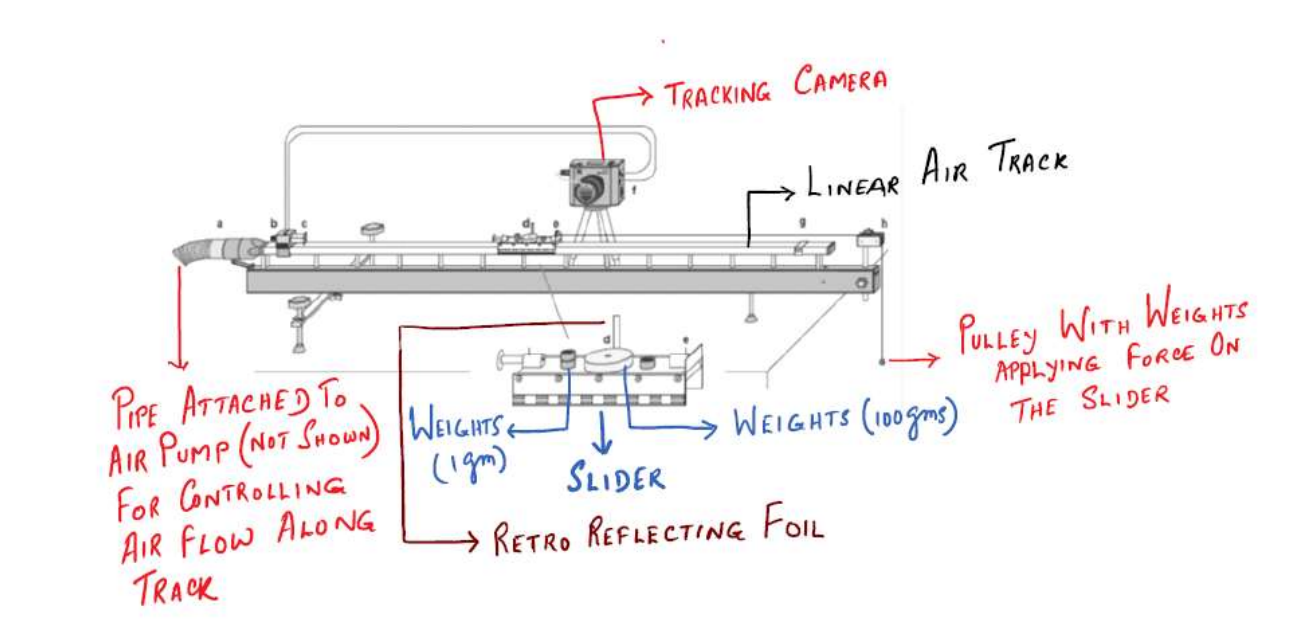
\includegraphics[scale=0.5]{exp setup}
		\caption{Experimental Setup}
		\label{figure:exp}%labeling the image
	\end{figure}

	\section{Objectives}
	According to Newton’s Second Law of Motion, $F=ma$, where $F$ is the force, $m$ is 
	the mass of the object and $a$ is the acceleration of the object. To verify this law using the air-track system, we need to show that when the mass of the object is fixed, the acceleration of 
	the object is proportional to the applied Force. Also, when the applied force is kept constant 
	and the mass of the object is varied, the acceleration varies inversely with mass.
	
	\section{Theory}
	\subsection{Newton’s Second Law}
	According to Newton’s Second law of motion, the force $F$ required to move a 
	body of given mass with an acceleration a is proportional to the acceleration $a$ 
	i.e., $$F \propto a$$
	Also, the force $F$ required to move a body of mass m with a given acceleration 
	$a$ is proportional to the mass $m$, given as, $$F \propto m$$
	Combining the two proportionality relations we get, $$F\propto ma \Rightarrow F = kma$$
	Here K is a constant of proportionality and the unit and dimension for force are 
	chosen such that $k$ has a unit magnitude and is dimensionless . So, $$F=ma$$
	
	\subsection{Working Formulae}
	Let $T$ be the tension in the string connecting the slider and the hanging 
	weights. This $T$ is the force $F$ acting on the slider system :
	For the (vertical) motion of the hanging weight $m$, $$T = mg - ma$$
	For horizontal motion of the system $M$,
	$$T = Ma + \mu Mg$$
	where, $g=$Acceleration due to gravity(=9.8 m/s)\\
	$\mu =$Coefficient of friction\\
	$M=$Mass of the sliding system\\ 
	$m=$Mass of the hanging weights\\[7pt]
	Combining the above two expressions and rearranging, we get,
	$$a = \frac{mg-\mu Mg}{m+M} = \frac{g(m-\mu M)}{m+M}$$
	and since we are using an Air Track we may assume $\mu = 0$. Thus, we have,
	$$a = \frac{mg}{m+M}$$
	and,
	$$T = \frac{Mmg}{m+M}+ M = F$$
	
	\section{Data Plotting and Analysis}
		\subsection{Fixed Mass Case} In this case, the combined 
		mass of the slider and the hanging weights (i.e. 
		$M+m$) has been kept constant and the experiment 
		has been repeated $6$ times with different values of 
		hanging weights($m$) as:\\
		4.13 g ,3.45 g, 2.76 g, 2.08 g, 1.39 g and 0.70 g \\
		Now we plot position, velocity and acceleration values against time from out 
		experimental data as below:
		
		\textbf{Displacement vs. Time Graph:-}
		
		\begin{figure}[H]
			\centering
			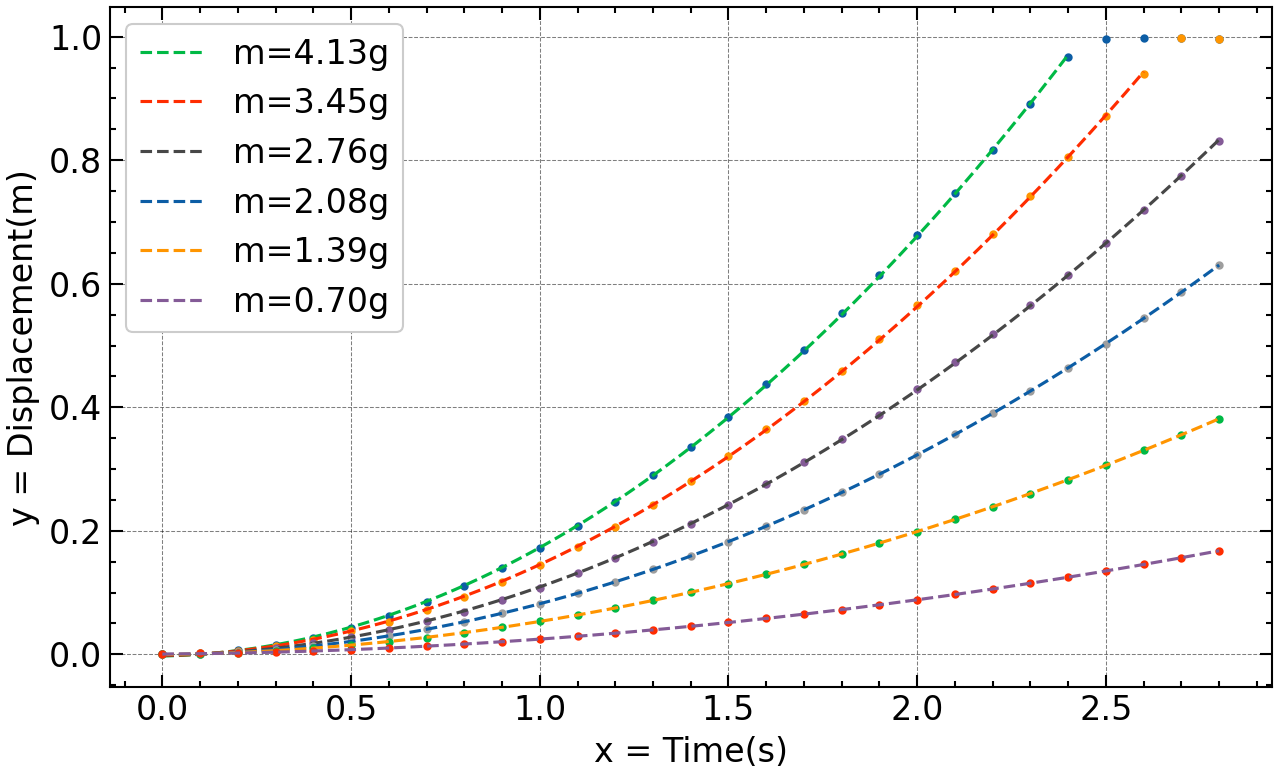
\includegraphics[scale=0.7]{displacement vs. time (fitted)}
			\caption{}
			\label{figure:disptime}%labeling the image
		\end{figure}
	
		\begin{table}[H]
			\centering
			\begin{tabular}{|c||c|}
				\hline
				Mass      & Polynomial Generated by Fitting Algorithm \\\hline\\
				m = 4.13g &  $0.1643 t^{2} + 0.01126 t - 0.002624$\\
				\hline\\
				m = 3.45g &  $0.135 t^{2} + 0.01245 t - 0.002142$\\
				\hline\\
				m = 2.76g &  $0.1043 t^{2} + 0.006136 t - 0.001242$\\
				\hline\\
				m = 2.08g & $0.07948 t^{2} + 0.002629 t - 0.0002204$\\
				\hline\\
				m = 1.39g &  $0.04593 t^{2} + 0.007786 t - 0.0004171$\\
				\hline\\
				m = 0.70g & $0.01974 t^{2} + 0.004472 t + 0.00046$\\ \hline                            
			\end{tabular}
		\caption{Polynomials generated by the Fitting Algorithm used}
		\label{table:ploy}
		\end{table}
	The acceleration $a$ can be calculated using the coefficient of $t^2$ according to the formula $\frac{1}{2}at^2 + vt + const.$
	
	\pagebreak
	
		Python Code used for plotting and curve - fitting: \\
		
		\begin{lstlisting}
			import matplotlib.pyplot as plt
			import numpy as np
			plt.style.use(['science', 'notebook', 'grid'])
			from scipy.optimize import curve_fit
			
			plt.figure(figsize=(10,6), dpi=150)
			
			time, disp = np.genfromtxt('xyz.csv',  dtype = 'float', delimiter = ',', unpack = True, usecols=[0,1])
			plt.plot(time, disp, 'o', ms=3)
			
			time, disp = np.genfromtxt('xyz.csv',  dtype = 'float', delimiter = ',', unpack = True, usecols=[0,1],
			skip_footer=4)
			z = np.polyfit(time, disp, 2)
			f = np.poly1d(z)
			time_opt = np.linspace(time[0], time[-1], 500)
			disp_opt = f(time_opt)
			
			print(f)
			
			plt.plot(time_opt, disp_opt, '--', lw=1.5, label='m=4.13g')
			
			time, disp = np.genfromtxt('xyz.csv',  dtype = 'float', delimiter = ',', unpack = True, usecols=[0,2])
			plt.plot(time, disp, 'o', ms=3)
			
			time, disp = np.genfromtxt('xyz.csv',  dtype = 'float', delimiter = ',', unpack = True, usecols=[0,2],
			 skip_footer=2)
			z = np.polyfit(time, disp, 2)
			f = np.poly1d(z)
			time_opt = np.linspace(time[0], time[-1], 500)
			disp_opt = f(time_opt)
			
			print(f)
			
			plt.plot(time_opt, disp_opt, '--', lw=1.5, label='m=3.45g')
			
			time, disp = np.genfromtxt('xyz.csv',  dtype = 'float', delimiter = ',', unpack = True, usecols=[0,3])
			plt.plot(time, disp, 'o', ms=3)
			
			time, disp = np.genfromtxt('xyz.csv',  dtype = 'float', delimiter = ',', unpack = True, usecols=[0,3])
			z = np.polyfit(time, disp, 2)
			f = np.poly1d(z)
			time_opt = np.linspace(time[0], time[-1], 500)
			disp_opt = f(time_opt)
			
			print(f)
			
			plt.plot(time_opt, disp_opt, '--', lw=1.5, label='m=2.76g')
			
			time, disp = np.genfromtxt('xyz.csv',  dtype = 'float', delimiter = ',', unpack = True, usecols=[0,4])
			plt.plot(time, disp, 'o', ms=3)
			
			time, disp = np.genfromtxt('xyz.csv',  dtype = 'float', delimiter = ',', unpack = True, usecols=[0,4])
			z = np.polyfit(time, disp, 2)
			f = np.poly1d(z)
			time_opt = np.linspace(time[0], time[-1], 500)
			disp_opt = f(time_opt)
			
			print(f)
			
			plt.plot(time_opt, disp_opt, '--', lw=1.5, label='m=2.08g')
			
			time, disp = np.genfromtxt('xyz.csv',  dtype = 'float', delimiter = ',', unpack = True, usecols=[0,5])
			plt.plot(time, disp, 'o', ms=3)
			
			time, disp = np.genfromtxt('xyz.csv',  dtype = 'float', delimiter = ',', unpack = True, usecols=[0,5])
			z = np.polyfit(time, disp, 2)
			f = np.poly1d(z)
			time_opt = np.linspace(time[0], time[-1], 500)
			disp_opt = f(time_opt)
			
			print(f)
			
			plt.plot(time_opt, disp_opt, '--', lw=1.5, label='m=1.39g')
			
			time, disp = np.genfromtxt('xyz.csv',  dtype = 'float', delimiter = ',', unpack = True, usecols=[0,6])
			plt.plot(time, disp, 'o', ms = 3)
			
			time, disp = np.genfromtxt('xyz.csv',  dtype = 'float', delimiter = ',', unpack = True, usecols=[0,6])
			z = np.polyfit(time, disp, 2)
			f = np.poly1d(z)
			time_opt = np.linspace(time[0], time[-1], 500)
			disp_opt = f(time_opt)
			
			print(f)
			
			plt.plot(time_opt, disp_opt, '--', lw=1.5, label='m=0.70g')
			plt.xlabel('x = Time(s)')
			plt.ylabel('y = Displacement(m)')
			plt.legend()
			plt.savefig('displacement vs. time (fitted).png')
			plt.show()
		\end{lstlisting}
	 
	 After this step, the formula $v(t+\frac{\delta t}{2}) = \frac{[x(t+\delta t) - x(t)]}{\delta t}$ was used to calculate the velocities for the corresponding displacements in time $\delta t = 0.1s$.
	 
	 \pagebreak
	 
	 The python code used to generate a sample .csv file with velocities is as follows:
	 
	 \begin{lstlisting}
	 	import csv
	 	import random
	 	time, disp = np.loadtxt('xyz.csv', dtype = 'float', delimiter = ',', unpack = True, usecols = [0,1])
	 	time = time + (0.1/2)
	 	vel = []
	 	vel.append([])
	 	vel.append([])
	 	vel.append([])
	 	vel.append([])
	 	vel.append([])
	 	vel.append([])
	 	vel.append([])
	 	for i in range (0, len(time)-1):
	 	vel[0].append(float((disp[i+1] - disp[i])/0.1))
	 	time, disp = np.loadtxt('xyz.csv', dtype = 'float', delimiter = ',', unpack = True, usecols = [0,2])
	 	for i in range (0, len(time)-1):
	 	vel[1].append(float((disp[i+1] - disp[i])/0.1))
	 	time, disp = np.loadtxt('xyz.csv', dtype = 'float', delimiter = ',', unpack = True, usecols = [0,3])
	 	for i in range (0, len(time)-1):
	 	vel[2].append(float((disp[i+1] - disp[i])/0.1))
	 	time, disp = np.loadtxt('xyz.csv', dtype = 'float', delimiter = ',', unpack = True, usecols = [0,4])
	 	for i in range (0, len(time)-1):
	 	vel[3].append(float((disp[i+1] - disp[i])/0.1))
	 	time, disp = np.loadtxt('xyz.csv', dtype = 'float', delimiter = ',', unpack = True, usecols = [0,5])
	 	for i in range (0, len(time)-1):
	 	vel[4].append(float((disp[i+1] - disp[i])/0.1))
	 	time, disp = np.loadtxt('xyz.csv', dtype = 'float', delimiter = ',', unpack = True, usecols = [0,6])
	 	for i in range (0, len(time)-1):
	 	vel[5].append(float((disp[i+1] - disp[i])/0.1))
	 	
	 	
	 	with open('velocity.csv', 'w') as f:
	 	    writer = csv.writer(f)
	 	    writer.writerow(vel)
	 \end{lstlisting}
	 	
	 	After this step, playing around with MS-Excel helped me get the .csv file in the desired format for plotting the graphs.
	 	
	 	Finally, the velocity and time data looked like this:
	 	
	 	\begin{table}[!ht]
	 		\centering
	 		\begin{tabular}{|l|l|l|l|l|l|l|}
	 			\hline
	 			0.05 & 0.01 & 0.01 & 0.005 & 0.005 & 0.005 & 0.005 \\ \hline
	 			0.15 & 0.052 & 0.047 & 0.034 & 0.026 & 0.018 & 0.006 \\ \hline
	 			0.25 & 0.085 & 0.072 & 0.054 & 0.039 & 0.029 & 0.012 \\ \hline
	 			0.35 & 0.118 & 0.103 & 0.08 & 0.059 & 0.038 & 0.019 \\ \hline
	 			0.45 & 0.155 & 0.134 & 0.098 & 0.072 & 0.049 & 0.02 \\ \hline
	 			0.55 & 0.191 & 0.157 & 0.121 & 0.093 & 0.059 & 0.026 \\ \hline
	 			0.65 & 0.226 & 0.188 & 0.136 & 0.105 & 0.07 & 0.031 \\ \hline
	 			0.75 & 0.258 & 0.214 & 0.16 & 0.121 & 0.077 & 0.036 \\ \hline
	 			0.85 & 0.293 & 0.242 & 0.185 & 0.137 & 0.09 & 0.041 \\ \hline
	 			0.95 & 0.325 & 0.268 & 0.201 & 0.154 & 0.098 & 0.041 \\ \hline
	 			1.05 & 0.358 & 0.298 & 0.232 & 0.17 & 0.103 & 0.047 \\ \hline
	 			1.15 & 0.394 & 0.33 & 0.247 & 0.186 & 0.114 & 0.051 \\ \hline
	 			1.25 & 0.427 & 0.353 & 0.268 & 0.206 & 0.123 & 0.054 \\ \hline
	 			1.35 & 0.461 & 0.378 & 0.288 & 0.216 & 0.129 & 0.057 \\ \hline
	 			1.45 & 0.492 & 0.41 & 0.312 & 0.232 & 0.139 & 0.062 \\ \hline
	 			1.55 & 0.525 & 0.435 & 0.332 & 0.25 & 0.149 & 0.064 \\ \hline
	 			1.65 & 0.557 & 0.458 & 0.353 & 0.265 & 0.16 & 0.07 \\ \hline
	 			1.75 & 0.59 & 0.49 & 0.373 & 0.281 & 0.165 & 0.072 \\ \hline
	 			1.85 & 0.618 & 0.512 & 0.394 & 0.296 & 0.18 & 0.077 \\ \hline
	 			1.95 & 0.646 & 0.544 & 0.412 & 0.314 & 0.188 & 0.082 \\ \hline
	 			2.05 & 0.68 & 0.564 & 0.436 & 0.33 & 0.198 & 0.088 \\ \hline
	 			2.15 & 0.706 & 0.589 & 0.453 & 0.342 & 0.204 & 0.087 \\ \hline
	 			2.25 & 0.733 & 0.616 & 0.474 & 0.361 & 0.214 & 0.093 \\ \hline
	 			2.35 & 0.76 & 0.636 & 0.494 & 0.376 & 0.224 & 0.098 \\ \hline
	 			2.45 & 0.304 & 0.662 & 0.51 & 0.391 & 0.234 & 0.103 \\ \hline
	 			2.55 & 0.005 & 0.68 & 0.536 & 0.407 & 0.242 & 0.103 \\ \hline
	 			2.65 & 0 & 0.579 & 0.551 & 0.422 & 0.25 & 0.108 \\ \hline
	 			2.75 & -0.01 & -0.005 & 0.569 & 0.436 & 0.26 & 0.114 \\ \hline
	 		\end{tabular}
	 		\caption{Time and Velocity}
	 		\label{veltime}
	 	\end{table}
 	
 	Here, the first column represents time and the rest represent velocities at different instances of time with the different masses.
 	
 	\pagebreak
 	
 	
 	\textbf{Velocity vs. Time Graphs:-}
 	
 	\begin{figure}[H]
 		\centering
 		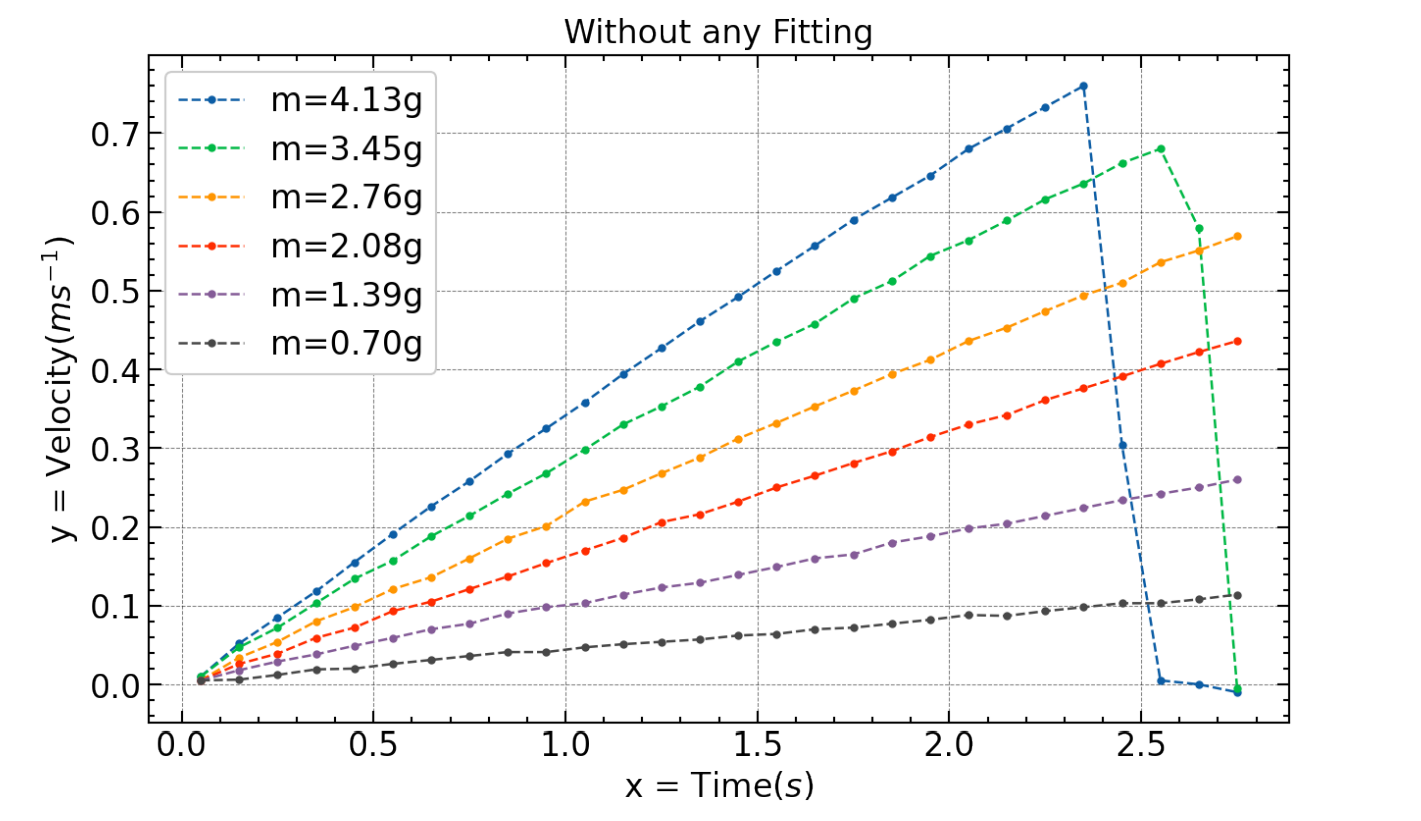
\includegraphics[scale=0.6]{Screenshot 2022-03-07 185137}
 		\caption{Velocity vs. Time}
 		\label{figure:veltimenf}%labeling the image
 	\end{figure}
 
 	\textbf{NOTE}: The abrupt enormous decrease in the velocity values towards the right represents the 
 	slider hitting the boundary.
 
 	Python code used for plotting:
 	
 	\begin{lstlisting}
 		import matplotlib.pyplot as plt
 		import numpy as np
 		plt.style.use(['science', 'notebook', 'grid'])
 		from scipy.optimize import curve_fit
 		
 		plt.figure(figsize=(10,6), dpi=150)
 		
 		time, velo = np.genfromtxt('velocity.csv',  dtype = 'float', delimiter = ',', unpack = True, usecols=[0,1])
 		plt.plot(time, velo, 'o--',lw=1.2, ms=3, label='m=4.13g')
 		
 		
 		time, velo = np.genfromtxt('velocity.csv',  dtype = 'float', delimiter = ',', unpack = True, usecols=[0,2])
 		plt.plot(time, velo, 'o--',lw=1.2, ms=3, label='m=3.45g')
 		
 		
 		time, velo = np.genfromtxt('velocity.csv',  dtype = 'float', delimiter = ',', unpack = True, usecols=[0,3])
 		plt.plot(time, velo, 'o--',lw=1.2, ms=3, label='m=2.76g')
 		
 		
 		time, velo = np.genfromtxt('velocity.csv',  dtype = 'float', delimiter = ',', unpack = True, usecols=[0,4])
 		plt.plot(time, velo, 'o--',lw=1.2, ms=3, label='m=2.08g')
 		
 		
 		time, velo = np.genfromtxt('velocity.csv',  dtype = 'float', delimiter = ',', unpack = True, usecols=[0,5])
 		plt.plot(time, velo, 'o--',lw=1.2, ms=3, label='m=1.39g')
 		
 		
 		time, velo = np.genfromtxt('velocity.csv',  dtype = 'float', delimiter = ',', unpack = True, usecols=[0,6])
 		plt.plot(time, velo, 'o--',lw=1.2, ms = 3, label='m=0.70g')
 		
 		plt.title('Without any Fitting')
 		plt.xlabel('x = Time($s$)')
 		plt.ylabel(r'y = Velocity($ms^{-1}$)')
 		plt.legend()
 		plt.savefig('vel vs. time (no-fit).png')
 		plt.show()
 	\end{lstlisting}
 
 	\begin{figure}[H]
 		\centering
 		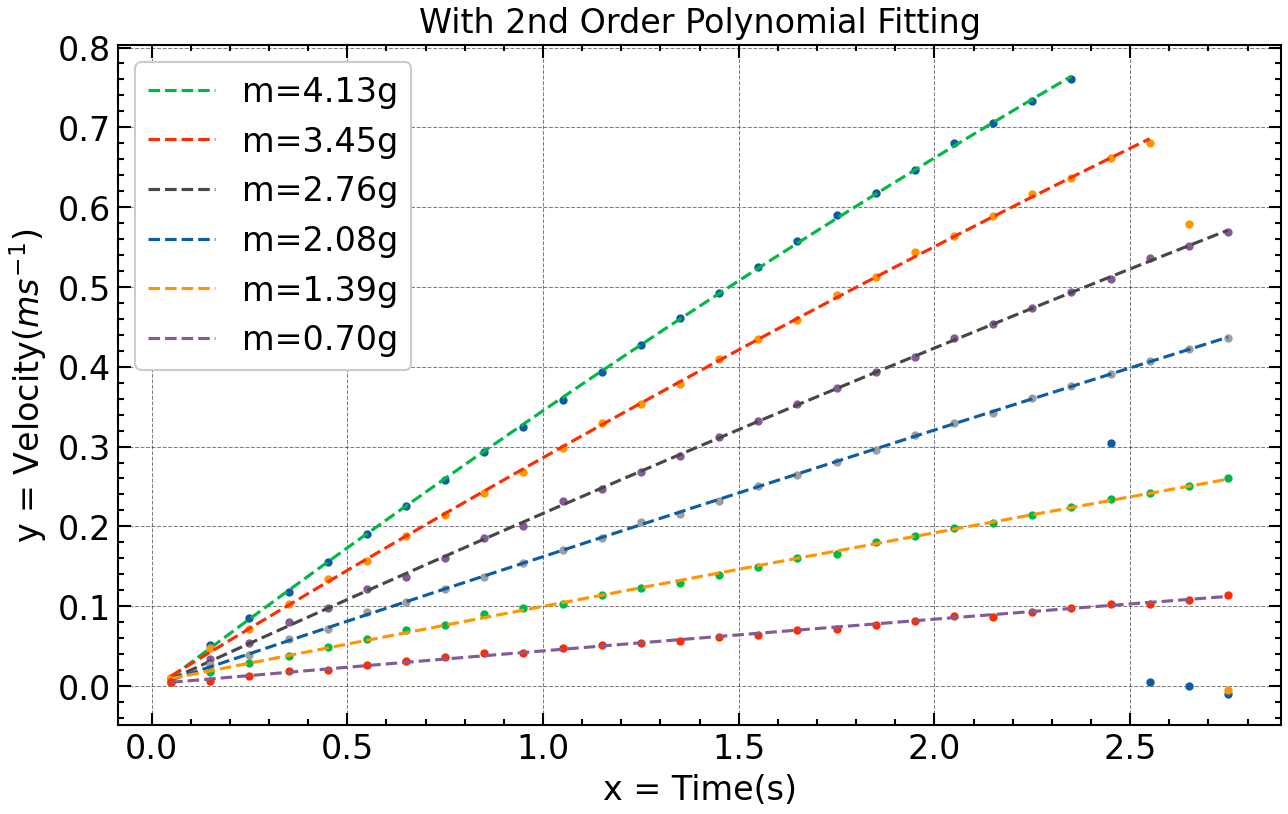
\includegraphics[scale=0.7]{vel vs. time (with fit).png}
 		\caption{Velocity vs. Time}
 		\label{figure:veltimef}%labeling the image
 	\end{figure}
 
 	Python Code used for fitting:
 	
 	\begin{lstlisting}
 		import matplotlib.pyplot as plt
 		import numpy as np
 		plt.style.use(['science', 'notebook', 'grid'])
 		from scipy.optimize import curve_fit
 		
 		plt.figure(figsize=(10,6), dpi=150)
 		
 		# Here, consider that the variable disp is representing velocity
 		
 		time, disp = np.genfromtxt('velocity.csv',  dtype = 'float', delimiter = ',', unpack = True, usecols=[0,1])
 		plt.plot(time, disp, 'o', ms=3)
 		
 		time, disp = np.genfromtxt('velocity.csv',  dtype = 'float', delimiter = ',', unpack = True, usecols=[0,1],
 		skip_footer=4)
 		z = np.polyfit(time, disp, 2)
 		f = np.poly1d(z)
 		time_opt = np.linspace(time[0], time[-1], 500)
 		disp_opt = f(time_opt)
 		
 		plt.plot(time_opt, disp_opt, '--', lw=1.5, label='m=4.13g')
 		
 		time, disp = np.genfromtxt('velocity.csv',  dtype = 'float', delimiter = ',', unpack = True, usecols=[0,2])
 		plt.plot(time, disp, 'o', ms=3)
 		
 		time, disp = np.genfromtxt('velocity.csv',  dtype = 'float', delimiter = ',', unpack = True, usecols=[0,2],
 		skip_footer=2)
 		z = np.polyfit(time, disp, 2)
 		f = np.poly1d(z)
 		time_opt = np.linspace(time[0], time[-1], 500)
 		disp_opt = f(time_opt)
 		
 		plt.plot(time_opt, disp_opt, '--', lw=1.5, label='m=3.45g')
 		
 		time, disp = np.genfromtxt('velocity.csv',  dtype = 'float', delimiter = ',', unpack = True, usecols=[0,3])
 		plt.plot(time, disp, 'o', ms=3)
 		
 		time, disp = np.genfromtxt('velocity.csv',  dtype = 'float', delimiter = ',', unpack = True, usecols=[0,3])
 		z = np.polyfit(time, disp, 2)
 		f = np.poly1d(z)
 		time_opt = np.linspace(time[0], time[-1], 500)
 		disp_opt = f(time_opt)
 		
 		plt.plot(time_opt, disp_opt, '--', lw=1.5, label='m=2.76g')
 		
 		time, disp = np.genfromtxt('velocity.csv',  dtype = 'float', delimiter = ',', unpack = True, usecols=[0,4])
 		plt.plot(time, disp, 'o', ms=3)
 		
 		time, disp = np.genfromtxt('velocity.csv',  dtype = 'float', delimiter = ',', unpack = True, usecols=[0,4])
 		z = np.polyfit(time, disp, 2)
 		f = np.poly1d(z)
 		time_opt = np.linspace(time[0], time[-1], 500)
 		disp_opt = f(time_opt)
 		
 		plt.plot(time_opt, disp_opt, '--', lw=1.5, label='m=2.08g')
 		
 		time, disp = np.genfromtxt('velocity.csv',  dtype = 'float', delimiter = ',', unpack = True, usecols=[0,5])
 		plt.plot(time, disp, 'o', ms=3)
 		
 		time, disp = np.genfromtxt('velocity.csv',  dtype = 'float', delimiter = ',', unpack = True, usecols=[0,5])
 		z = np.polyfit(time, disp, 2)
 		f = np.poly1d(z)
 		time_opt = np.linspace(time[0], time[-1], 500)
 		disp_opt = f(time_opt)
 		
 		plt.plot(time_opt, disp_opt, '--', lw=1.5, label='m=1.39g')
 		
 		time, disp = np.genfromtxt('velocity.csv',  dtype = 'float', delimiter = ',', unpack = True, usecols=[0,6])
 		plt.plot(time, disp, 'o', ms = 3)
 		
 		time, disp = np.genfromtxt('velocity.csv',  dtype = 'float', delimiter = ',', unpack = True, usecols=[0,6])
 		z = np.polyfit(time, disp, 2)
 		f = np.poly1d(z)
 		time_opt = np.linspace(time[0], time[-1], 500)
 		disp_opt = f(time_opt)
 		
 		plt.plot(time_opt, disp_opt, '--', lw=1.5, label='m=0.70g')
 		plt.title('With 2nd Order Polynomial Fitting')
 		plt.xlabel('x = Time(s)')
 		plt.ylabel(r'y = Velocity($ms^{-1}$)')
 		plt.legend()
 		plt.savefig('vel vs. time (with fit).png')
 		plt.show()
 	\end{lstlisting}
 
 	After this, I calculated acceleration using the formula $a(t) = \frac{[x(t+dt) + x(t-dt) - 2 x(t)]}{dt^2}$ and wrote it into a .csv file following the same process as was done in the velocity case. The final product looks as follows:
 	
 	\begin{table}[!ht]
 		\centering
 		\begin{tabular}{|l|l|l|l|l|l|l|}
 			\hline
 			0 & 0.42 & 0.37 & 0.29 & 0.21 & 0.13 & 0.01 \\ \hline
 			0.1 & 0.33 & 0.25 & 0.2 & 0.13 & 0.11 & 0.06 \\ \hline
 			0.2 & 0.33 & 0.31 & 0.26 & 0.2 & 0.09 & 0.07 \\ \hline
 			0.3 & 0.37 & 0.31 & 0.18 & 0.13 & 0.11 & 0.01 \\ \hline
 			0.4 & 0.36 & 0.23 & 0.23 & 0.21 & 0.1 & 0.06 \\ \hline
 			0.5 & 0.35 & 0.31 & 0.15 & 0.12 & 0.11 & 0.05 \\ \hline
 			0.6 & 0.32 & 0.26 & 0.24 & 0.16 & 0.07 & 0.05 \\ \hline
 			0.7 & 0.35 & 0.28 & 0.25 & 0.16 & 0.13 & 0.05 \\ \hline
 			0.8 & 0.32 & 0.26 & 0.16 & 0.17 & 0.08 & 0 \\ \hline
 			0.9 & 0.33 & 0.3 & 0.31 & 0.16 & 0.05 & 0.06 \\ \hline
 			1 & 0.36 & 0.32 & 0.15 & 0.16 & 0.11 & 0.04 \\ \hline
 			1.1 & 0.33 & 0.23 & 0.21 & 0.2 & 0.09 & 0.03 \\ \hline
 			1.2 & 0.34 & 0.25 & 0.2 & 0.1 & 0.06 & 0.03 \\ \hline
 			1.3 & 0.31 & 0.32 & 0.24 & 0.16 & 0.1 & 0.05 \\ \hline
 			1.4 & 0.33 & 0.25 & 0.2 & 0.18 & 0.1 & 0.02 \\ \hline
 			1.5 & 0.32 & 0.23 & 0.21 & 0.15 & 0.11 & 0.06 \\ \hline
 			1.6 & 0.33 & 0.32 & 0.2 & 0.16 & 0.05 & 0.02 \\ \hline
 			1.7 & 0.28 & 0.22 & 0.21 & 0.15 & 0.15 & 0.05 \\ \hline
 			1.8 & 0.28 & 0.32 & 0.18 & 0.18 & 0.08 & 0.05 \\ \hline
 			1.9 & 0.34 & 0.2 & 0.24 & 0.16 & 0.1 & 0.06 \\ \hline
 			2 & 0.26 & 0.25 & 0.17 & 0.12 & 0.06 & -0.01 \\ \hline
 			2.1 & 0.27 & 0.27 & 0.21 & 0.19 & 0.1 & 0.06 \\ \hline
 			2.2 & 0.27 & 0.2 & 0.2 & 0.15 & 0.1 & 0.05 \\ \hline
 			2.3 & -4.56 & 0.26 & 0.16 & 0.15 & 0.1 & 0.05 \\ \hline
 			2.4 & -2.99 & 0.18 & 0.26 & 0.16 & 0.08 & 0 \\ \hline
 			2.5 & -0.05 & -1.01 & 0.15 & 0.15 & 0.08 & 0.05 \\ \hline
 			2.6 & -0.1 & -5.84 & 0.18 & 0.14 & 0.1 & 0.06 \\ \hline
 		\end{tabular}
 		\caption{Time and Acceleration}
 		\label{acctime}
 	\end{table}
 
 	 Here also, the first column represents time and the rest represent accelerations at different time stamps for the different masses considered.
 	 
 	 \pagebreak
 
 	\textbf{Acceleration vs. Time Graphs:-}
 	
 	\begin{figure}[H]
 		\centering
 		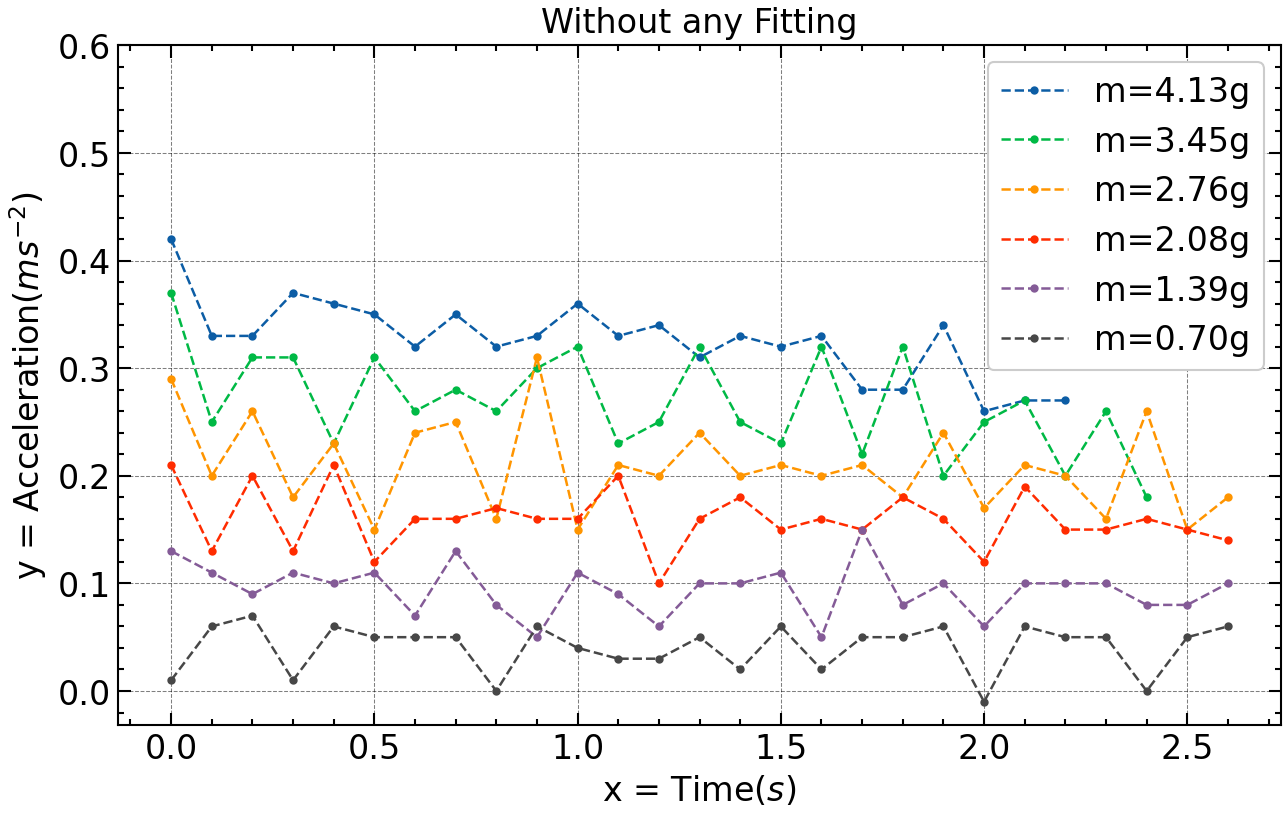
\includegraphics[scale=0.7]{acc vs. time (no-fit).png}
 		\caption{Acceleration vs. Time}
 		\label{figure:acctimenf}%labeling the image
 	\end{figure}
 
 	Again, python code used for plotting this,
 	
 	\begin{lstlisting}
 		import matplotlib.pyplot as plt
 		import numpy as np
 		plt.style.use(['science', 'notebook', 'grid'])
 		from scipy.optimize import curve_fit
 		
 		plt.figure(figsize=(10,6), dpi=150)
 		
 		time, velo = np.genfromtxt('acceleration.csv',  dtype = 'float', delimiter = ',', unpack = True, usecols=[0,1], skip_footer=4)
 		plt.plot(time, velo, 'o--',lw=1.2, ms=3, label='m=4.13g')
 		
 		
 		time, velo = np.genfromtxt('acceleration.csv',  dtype = 'float', delimiter = ',', unpack = True, usecols=[0,2], skip_footer=2)
 		plt.plot(time, velo, 'o--',lw=1.2, ms=3, label='m=3.45g')
 		
 		
 		time, velo = np.genfromtxt('acceleration.csv',  dtype = 'float', delimiter = ',', unpack = True, usecols=[0,3])
 		plt.plot(time, velo, 'o--',lw=1.2, ms=3, label='m=2.76g')
 		
 		
 		time, velo = np.genfromtxt('acceleration.csv',  dtype = 'float', delimiter = ',', unpack = True, usecols=[0,4])
 		plt.plot(time, velo, 'o--',lw=1.2, ms=3, label='m=2.08g')
 		
 		
 		time, velo = np.genfromtxt('acceleration.csv',  dtype = 'float', delimiter = ',', unpack = True, usecols=[0,5])
 		plt.plot(time, velo, 'o--',lw=1.2, ms=3, label='m=1.39g')
 		
 		
 		time, velo = np.genfromtxt('acceleration.csv',  dtype = 'float', delimiter = ',', unpack = True, usecols=[0,6])
 		plt.plot(time, velo, 'o--',lw=1.2, ms = 3, label='m=0.70g')
 		
 		plt.ylim(top = 0.6)
 		plt.title('Without any Fitting')
 		plt.xlabel('x = Time($s$)')
 		plt.ylabel(r'y = Acceleration($ms^{-2}$)')
 		plt.legend()
 		plt.savefig('acc vs. time (no-fit).png')
 		plt.show()
 	\end{lstlisting}
 
 	\pagebreak
 
 	\textbf{Force vs. Acceleration Graph:-}
 	
 	\begin{figure}[H]
 		\centering
 		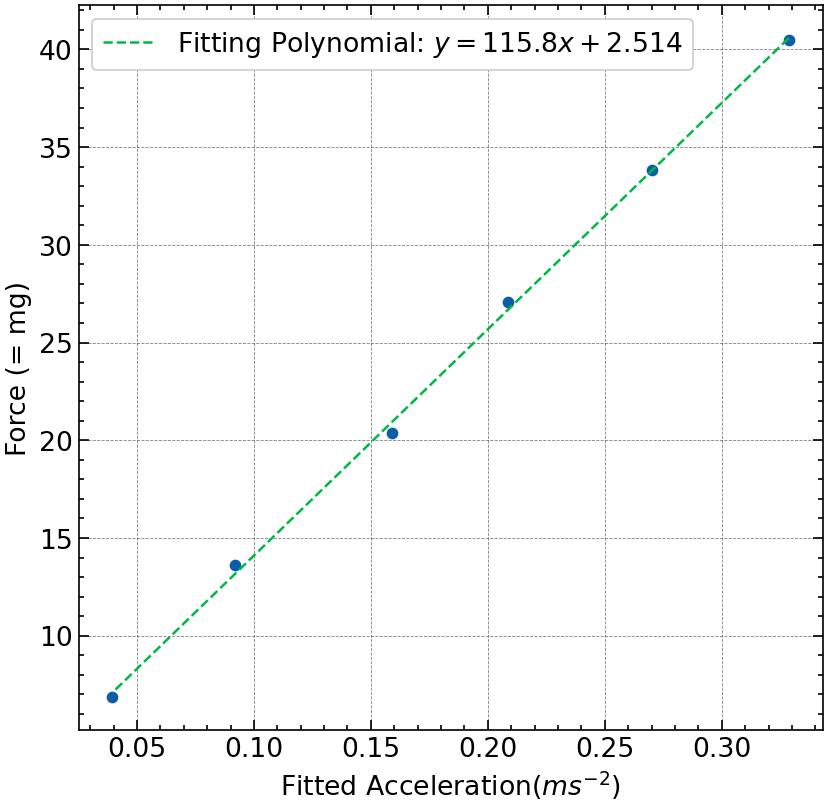
\includegraphics[scale=0.8]{final.png}
 		\caption{Force vs. Acceleration}
 		\label{figure:force}%labeling the image
 	\end{figure}
 
 	The Force vs Acceleration graph is obtained as a Linear fit, thus, Newton’s Second Law 
 	of Motion is verified for Fixed Mass Case .
 
 	The python code used for plotting this graph was:
 	
 	\begin{lstlisting}
 		import matplotlib.pyplot as plt
 		import numpy as np
 		plt.style.use(['science', 'notebook', 'grid'])
 		from scipy.optimize import curve_fit
 		
 		force = [4.13*9.8, 3.45*9.8, 2.76*9.8, 2.08*9.8, 1.39*9.8, 0.70*9.8]
 		accln = [0.3286, 0.27, 0.2086, 0.15896, 0.09186, 0.03948]
 		plt.figure(figsize=(8,8), dpi=120)
 		plt.plot(accln, force, 'o')
 		z, res, _, sing, _ = np.polyfit(accln, force, 1, full='True')
 		f = np.poly1d(z)
 		print ("Fitting polynomial =",f)
 		print ('Sum of Residual Values =',res)
 		print('Singluar Asymptomatic Errors =',sing)
 		accln_opt = np.linspace(accln[0], accln[-1], 500)
 		force_opt = f(accln_opt)
 		plt.xlabel ('Fitted Acceleration($ms^{-2}$)')
 		plt.ylabel ('Force (= mg)')
 		plt.plot(accln_opt, force_opt, '--', lw=1.5, label=r'Equation of fitted curve: $y = 115.8x + 2.514$')
 		plt.legend()
 		plt.savefig('final.png')
 		plt.show()
 	\end{lstlisting}
 
 	This is the final graph for the \texttt{Fixed Mass Case}.\\
 	
 	\subsection{Error Analysis for Fixed Mass Case: }
 	
 	The sum of residual values generated by the above code is:
 	$$\texttt{Sum\ of\ Residual\ Values} = 0.7136271$$
 	And the asymptotic errors in each of the parameters of the fitting polynomial is:
 	\begin{table}[!ht]
 		\centering
 		\begin{tabular}{|l|l|}
 			\hline
 			Parameters & Singular Asymptotic Error \\ \hline
 			a (or m) & 1.37086951 \\ \hline
 			b & 0.34744323 \\ \hline
 		\end{tabular}
 		\caption{Errors in parameters of Fitting Polynomial}
 		\label{error}
 	\end{table}
 
 	Total Mass (Theoretical Value) $= 92.52g + 4.13g = 96.65g (\pm 1.37086951\%)$\\
 	Total Mass (Measured Value from Graph) $= 115.8g$\\
 	$\Rightarrow$ Relative Error $= \frac{115.8-96.65}{96.65} \times 100\% = 19.8\%$
 	
 	\subsection{Fixed Force Case}
 	
 	In this case, the force $F$ (i.e tension $T$ in 
 	string) acting on the slider has been kept constant and the 
 	experiment has been repeated $4$ times with different values of mass 
 	of slider system $M$ (i.e. slider+additional weights on slider) as:\\
 	\begin{center}
 		400.61g, 300.47g, 200.29g and 100.01g \\
 		And mass of slider ($m_s$) = 92.52 g 
 	\end{center}
 
 	Now we plot position, velocity and acceleration values against time from 
 	out experimental data as below:
 	
 	\textbf{Displacement vs. Time Graph:-}
 	
 	\begin{figure}[H]
 		\centering
 		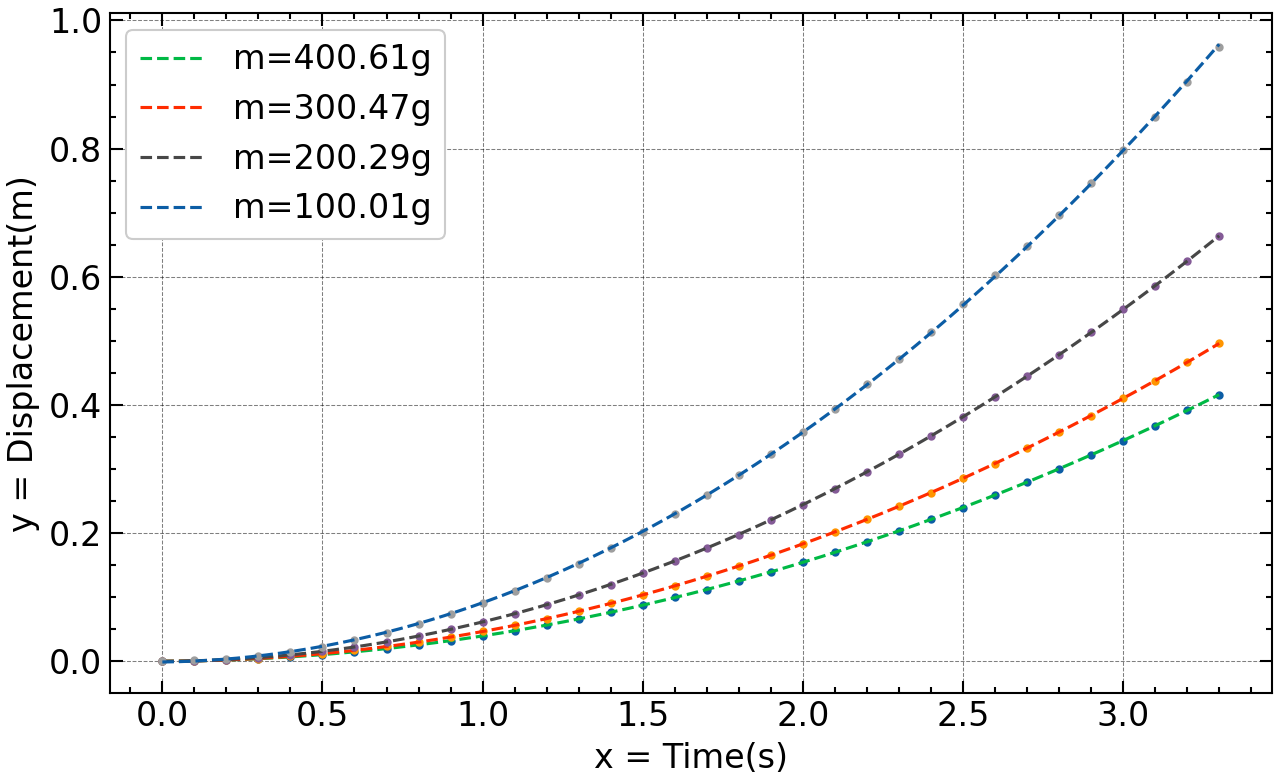
\includegraphics[scale=0.7]{displacement vs. time (fitter).png}
 		\caption{Displacement vs. Time}
 		\label{figure:displ}%labeling the image
 	\end{figure}
 	
 	\begin{table}[H]
 		\centering
 		\begin{tabular}{|c||c|}
 			\hline
 			Mass      & Polynomial Generated by Fitting Algorithm \\\hline\\
 			m = 400.61g &  $0.03764 t^2 + 0.00191 t - 0.0002409$ \\
 			\hline\\
 			m = 300.47g &  $0.04515 t^2 + 0.001345 t - 0.0003122$ \\
 			\hline\\
 			m = 200.29g &  $0.06083 t^2 + 0.0004967 t - 0.000176$ \\
 			\hline\\
 			m = 100.01g & $0.08683 t^2 + 0.005643 t - 0.001379$ \\
 			\hline                     
 		\end{tabular}
 		\caption{Polynomials generated by the Fitting Algorithm used}
 		\label{table:poly}
 	\end{table}
 
 	The acceleration $a$ can be calculated using the coefficient of $t^2$ according to the formula $\frac{1}{2}at^2 + vt + const.$
 	
 	The python code used for the plotting and data analysis is as follows:
 	
 	\begin{lstlisting}
 		import matplotlib.pyplot as plt
 		import numpy as np
 		plt.style.use(['science', 'notebook', 'grid'])
 		from scipy.optimize import curve_fit
 		
 		plt.figure(figsize=(10,6), dpi=150)
 		
 		time, disp = np.genfromtxt('displacement.csv',  dtype = 'float', delimiter = ',', unpack = True,usecols=[0,1])
 		plt.plot(time, disp, 'o', ms=3)
 		
 		time, disp = np.genfromtxt('displacement.csv',  dtype = 'float', delimiter = ',', unpack = True,usecols=[0,1])
 		z = np.polyfit(time, disp, 2)
 		f = np.poly1d(z)
 		time_opt = np.linspace(time[0], time[-1], 500)
 		disp_opt = f(time_opt)
 		
 		print(f)
 		
 		plt.plot(time_opt, disp_opt, '--', lw=1.5, label='m=400.61g')
 		
 		time, disp = np.genfromtxt('displacement.csv',  dtype = 'float', delimiter = ',', unpack = True,usecols=[0,2])
 		plt.plot(time, disp, 'o', ms=3)
 		
 		time, disp = np.genfromtxt('displacement.csv',  dtype = 'float', delimiter = ',', unpack = True,usecols=[0,2])
 		z = np.polyfit(time, disp, 2)
 		f = np.poly1d(z)
 		time_opt = np.linspace(time[0], time[-1], 500)
 		disp_opt = f(time_opt)
 		
 		print(f)
 		
 		plt.plot(time_opt, disp_opt, '--', lw=1.5, label='m=300.47g')
 		
 		time, disp = np.genfromtxt('displacement.csv',  dtype = 'float', delimiter = ',', unpack = True,usecols=[0,3])
 		plt.plot(time, disp, 'o', ms=3)
 		
 		time, disp = np.genfromtxt('displacement.csv',  dtype = 'float', delimiter = ',', unpack = True,usecols=[0,3])
 		z = np.polyfit(time, disp, 2)
 		f = np.poly1d(z)
 		time_opt = np.linspace(time[0], time[-1], 500)
 		disp_opt = f(time_opt)
 		
 		print(f)
 		
 		plt.plot(time_opt, disp_opt, '--', lw=1.5, label='m=200.29g')
 		
 		time, disp = np.genfromtxt('displacement.csv',  dtype = 'float', delimiter = ',', unpack = True,usecols=[0,4])
 		plt.plot(time, disp, 'o', ms=3)
 		
 		time, disp = np.genfromtxt('displacement.csv',  dtype = 'float', delimiter = ',', unpack = True,usecols=[0,4])
 		z = np.polyfit(time, disp, 2)
 		f = np.poly1d(z)
 		time_opt = np.linspace(time[0], time[-1], 500)
 		disp_opt = f(time_opt)
 		
 		print(f)
 		
 		
 		
 		plt.plot(time_opt, disp_opt, '--', lw=1.5, label='m=100.01g')
 		plt.xlabel('x = Time(s)')
 		plt.ylabel('y = Displacement(m)')
 		plt.legend()
 		plt.savefig('displacement vs. time (fitter).png')
 		plt.show()
 	\end{lstlisting}
 
 	After this step, I used the following code to calculate velocity for each case using the formula $v(t+\frac{dt}{2}) = \frac{[x(t+dt) - x(t)]}{dt}$, and write it into a .csv file:
 	
 	\begin{lstlisting}
 		import csv
 		import random
 		time, disp = np.loadtxt('displacement.csv', dtype = 'float', delimiter = ',', unpack = True, usecols = [0,1])
 		time = time + (0.1/2)
 		vel = []
 		vel.append([])
 		vel.append([])
 		vel.append([])
 		vel.append([])
 		vel.append([])
 		vel.append([])
 		vel.append([])
 		for i in range (0, len(time)-1):
 		vel[0].append(float((disp[i+1] - disp[i])/0.1))
 		time, disp = np.loadtxt('displacement.csv', dtype = 'float', delimiter = ',', unpack = True, usecols = [0,2])
 		for i in range (0, len(time)-1):
 		vel[1].append(float((disp[i+1] - disp[i])/0.1))
 		time, disp = np.loadtxt('displacement.csv', dtype = 'float', delimiter = ',', unpack = True, usecols = [0,3])
 		for i in range (0, len(time)-1):
 		vel[2].append(float((disp[i+1] - disp[i])/0.1))
 		time, disp = np.loadtxt('displacement.csv', dtype = 'float', delimiter = ',', unpack = True, usecols = [0,4])
 		for i in range (0, len(time)-1):
 		vel[3].append(float((disp[i+1] - disp[i])/0.1))
 		
 		
 		with open('velocity1.csv', 'w') as f:
 		writer = csv.writer(f)
 		writer.writerow(vel)
 	\end{lstlisting}
 
 	After this, I played around with the data in MS-Excel, and the final data looks like this: 
 	
 	\begin{table}[!ht]
 		\centering
 		\begin{tabular}{|l|l|l|l|l|}
 			\hline
 			0.05 & 0.003 & 0.006 & 0.011 & 0.005 \\ \hline
 			0.15 & 0.015 & 0.015 & 0.015 & 0.026 \\ \hline
 			0.25 & 0.018 & 0.021 & 0.031 & 0.046 \\ \hline
 			0.35 & 0.028 & 0.036 & 0.044 & 0.062 \\ \hline
 			0.45 & 0.036 & 0.041 & 0.056 & 0.079 \\ \hline
 			0.55 & 0.044 & 0.051 & 0.067 & 0.101 \\ \hline
 			0.65 & 0.051 & 0.062 & 0.08 & 0.113 \\ \hline
 			0.75 & 0.06 & 0.067 & 0.093 & 0.136 \\ \hline
 			0.85 & 0.064 & 0.08 & 0.102 & 0.154 \\ \hline
 			0.95 & 0.075 & 0.087 & 0.116 & 0.17 \\ \hline
 			1.05 & 0.079 & 0.095 & 0.126 & 0.191 \\ \hline
 			1.15 & 0.088 & 0.106 & 0.142 & 0.205 \\ \hline
 			1.25 & 0.097 & 0.113 & 0.149 & 0.221 \\ \hline
 			1.35 & 0.103 & 0.123 & 0.164 & 0.242 \\ \hline
 			1.45 & 0.113 & 0.134 & 0.18 & 0.257 \\ \hline
 			1.55 & 0.119 & 0.139 & 0.186 & 0.278 \\ \hline
 			1.65 & 0.123 & 0.152 & 0.205 & 0.293 \\ \hline
 			1.75 & 0.134 & 0.159 & 0.211 & 0.314 \\ \hline
 			1.85 & 0.144 & 0.167 & 0.227 & 0.329 \\ \hline
 			1.95 & 0.149 & 0.18 & 0.239 & 0.345 \\ \hline
 			2.05 & 0.155 & 0.185 & 0.249 & 0.365 \\ \hline
 			2.15 & 0.164 & 0.196 & 0.265 & 0.384 \\ \hline
 			2.25 & 0.17 & 0.203 & 0.275 & 0.398 \\ \hline
 			2.35 & 0.18 & 0.214 & 0.289 & 0.417 \\ \hline
 			2.45 & 0.185 & 0.223 & 0.298 & 0.432 \\ \hline
 			2.55 & 0.196 & 0.232 & 0.311 & 0.448 \\ \hline
 			2.65 & 0.2 & 0.242 & 0.322 & 0.468 \\ \hline
 			2.75 & 0.209 & 0.249 & 0.334 & 0.478 \\ \hline
 			2.85 & 0.216 & 0.257 & 0.347 & 0.496 \\ \hline
 			2.95 & 0.223 & 0.268 & 0.358 & 0.512 \\ \hline
 			3.05 & 0.232 & 0.278 & 0.37 & 0.525 \\ \hline
 			3.15 & 0.239 & 0.285 & 0.381 & 0.54 \\ \hline
 			3.25 & 0.247 & 0.296 & 0.391 & 0.553 \\ \hline
 		\end{tabular}
 		\caption{Time and Velocity}
 		\label{vel1}
 	\end{table}
 
 	In this table, the first column represents different time stamps and the rest represent the velocities at those time stamps for the different masses considered.
 
 	\textbf{Velocity vs. Time Graph:-}
 	
 	\begin{figure}[H]
 		\centering
 		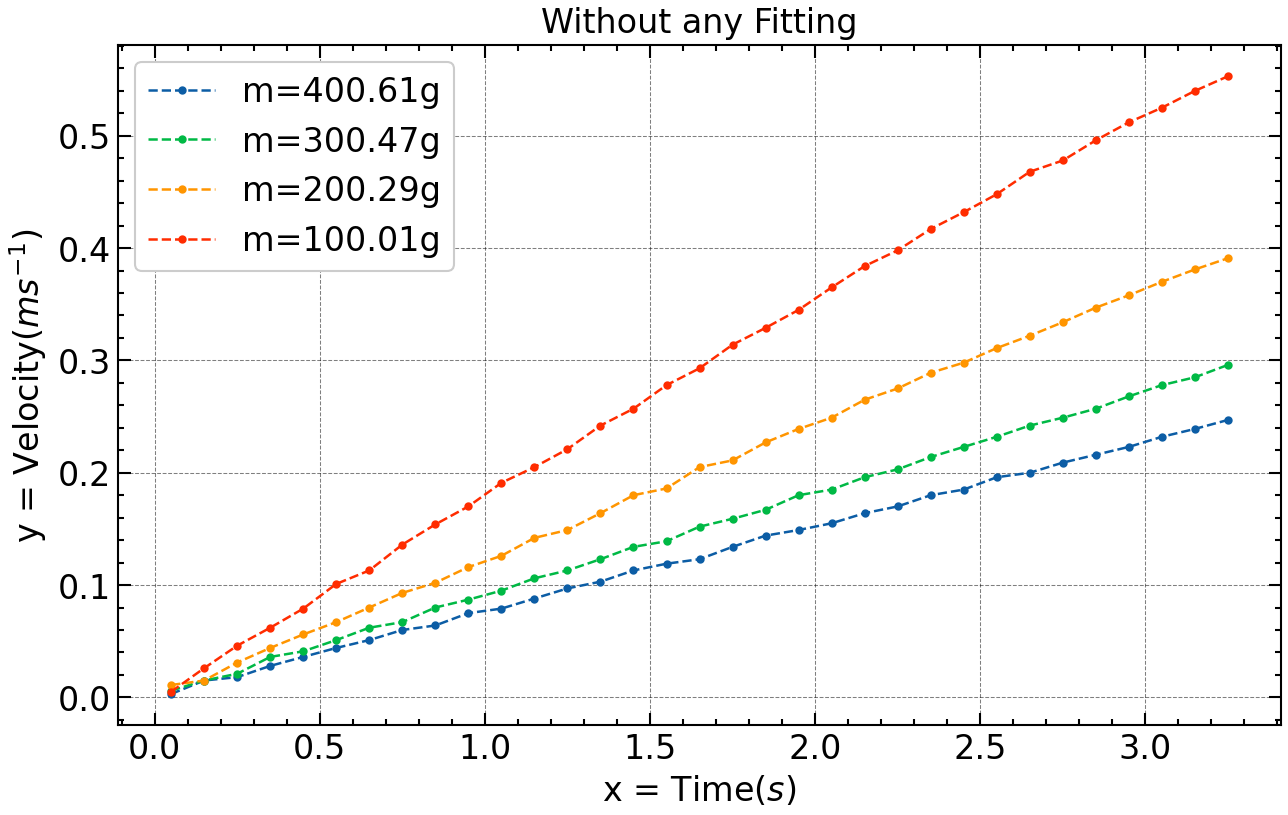
\includegraphics[scale=0.7]{vel vs. time (nfit).png}
 		\caption{Velocity vs. Time}
 		\label{figure:velnf}%labeling the image
 	\end{figure}
 
 Python Code used to plot this graph is as follows:
 
 \begin{lstlisting}
 	import matplotlib.pyplot as plt
 	import numpy as np
 	plt.style.use(['science', 'notebook', 'grid'])
 	from scipy.optimize import curve_fit
 	
 	plt.figure(figsize=(10,6), dpi=150)
 	
 	time, velo = np.genfromtxt('velocity1.csv',  dtype = 'float', delimiter = ',', unpack = True, usecols=[0,1])
 	plt.plot(time, velo, 'o--',lw=1.2, ms=3, label='m=400.61g')
 	
 	
 	time, velo = np.genfromtxt('velocity1.csv',  dtype = 'float', delimiter = ',', unpack = True, usecols=[0,2])
 	plt.plot(time, velo, 'o--',lw=1.2, ms=3, label='m=300.47g')
 	
 	
 	time, velo = np.genfromtxt('velocity1.csv',  dtype = 'float', delimiter = ',', unpack = True, usecols=[0,3])
 	plt.plot(time, velo, 'o--',lw=1.2, ms=3, label='m=200.29g')
 	
 	
 	time, velo = np.genfromtxt('velocity1.csv',  dtype = 'float', delimiter = ',', unpack = True, usecols=[0,4])
 	plt.plot(time, velo, 'o--',lw=1.2, ms=3, label='m=100.01g')
 	
 	plt.title('Without any Fitting')
 	plt.xlabel('x = Time($s$)')
 	plt.ylabel(r'y = Velocity($ms^{-1}$)')
 	plt.legend()
 	plt.savefig('vel vs. time (nfit).png')
 	plt.show()
 \end{lstlisting}

 \begin{figure}[H]
 	\centering
 	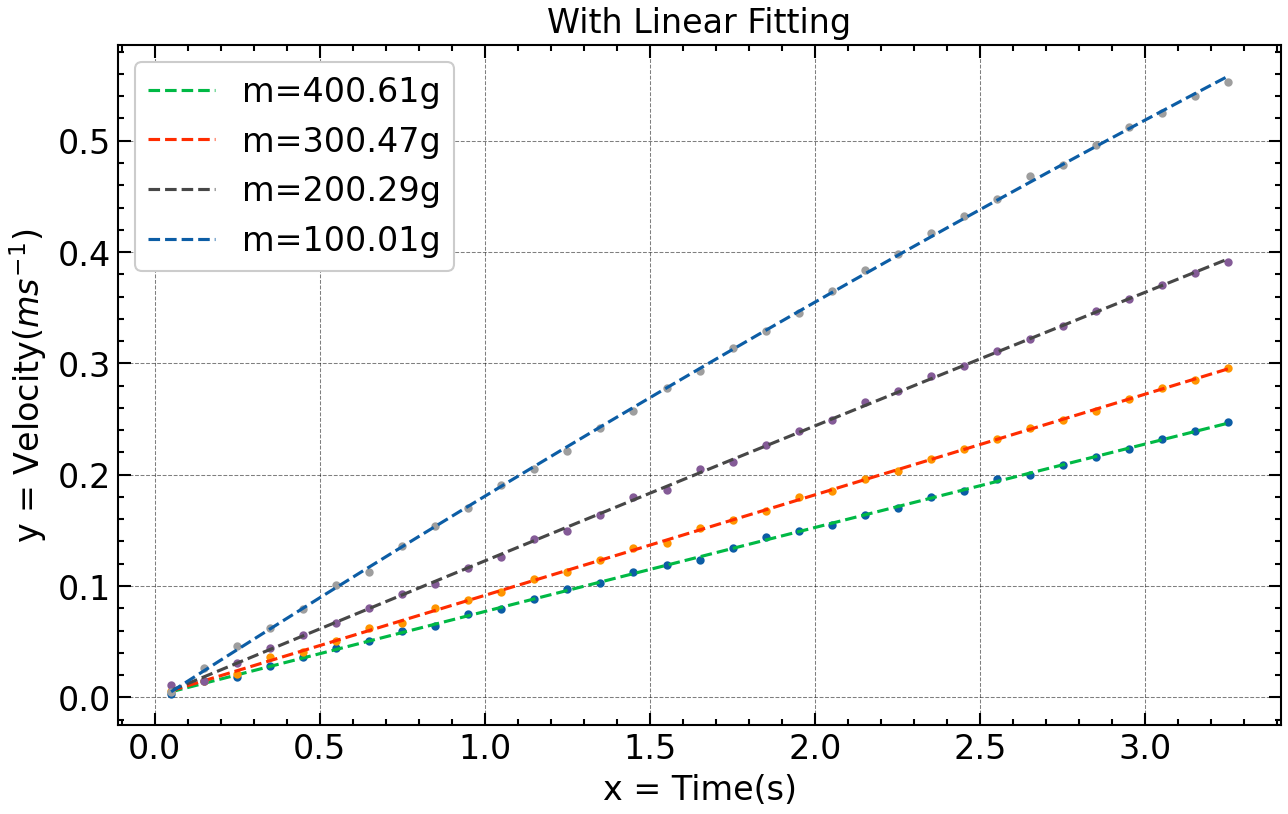
\includegraphics[scale=0.7]{vel vs. time (ffit).png}
 	\caption{Velocity vs. Time}
 	\label{figure:velf}%labeling the image
 \end{figure}

\pagebreak

The Python code used for plotting and fitting the above curve is as follows:

\begin{lstlisting}
	import matplotlib.pyplot as plt
	import numpy as np
	plt.style.use(['science', 'notebook', 'grid'])
	from scipy.optimize import curve_fit
	
	plt.figure(figsize=(10,6), dpi=150)
	
	# Here, consider that the variable disp is representing velocity
	
	time, disp = np.genfromtxt('velocity1.csv',  dtype = 'float', delimiter = ',', unpack = True, usecols=[0,1])
	plt.plot(time, disp, 'o', ms=3)
	
	time, disp = np.genfromtxt('velocity1.csv',  dtype = 'float', delimiter = ',', unpack = True, usecols=[0,1])
	z = np.polyfit(time, disp, 2)
	f = np.poly1d(z)
	time_opt = np.linspace(time[0], time[-1], 500)
	disp_opt = f(time_opt)
	
	plt.plot(time_opt, disp_opt, '--', lw=1.5, label='m=400.61g')
	
	time, disp = np.genfromtxt('velocity1.csv',  dtype = 'float', delimiter = ',', unpack = True, usecols=[0,2])
	plt.plot(time, disp, 'o', ms=3)
	
	time, disp = np.genfromtxt('velocity1.csv',  dtype = 'float', delimiter = ',', unpack = True, usecols=[0,2])
	z = np.polyfit(time, disp, 2)
	f = np.poly1d(z)
	time_opt = np.linspace(time[0], time[-1], 500)
	disp_opt = f(time_opt)
	
	plt.plot(time_opt, disp_opt, '--', lw=1.5, label='m=300.47g')
	
	time, disp = np.genfromtxt('velocity1.csv',  dtype = 'float', delimiter = ',', unpack = True, usecols=[0,3])
	plt.plot(time, disp, 'o', ms=3)
	
	time, disp = np.genfromtxt('velocity1.csv',  dtype = 'float', delimiter = ',', unpack = True, usecols=[0,3])
	z = np.polyfit(time, disp, 2)
	f = np.poly1d(z)
	time_opt = np.linspace(time[0], time[-1], 500)
	disp_opt = f(time_opt)
	
	plt.plot(time_opt, disp_opt, '--', lw=1.5, label='m=200.29g')
	
	time, disp = np.genfromtxt('velocity1.csv',  dtype = 'float', delimiter = ',', unpack = True, usecols=[0,4])
	plt.plot(time, disp, 'o', ms=3)
	
	time, disp = np.genfromtxt('velocity1.csv',  dtype = 'float', delimiter = ',', unpack = True, usecols=[0,4])
	z = np.polyfit(time, disp, 2)
	f = np.poly1d(z)
	time_opt = np.linspace(time[0], time[-1], 500)
	disp_opt = f(time_opt)
	
	plt.plot(time_opt, disp_opt, '--', lw=1.5, label='m=100.01g')
	
	plt.title('With Linear Fitting')
	plt.xlabel('x = Time(s)')
	plt.ylabel(r'y = Velocity($ms^{-1}$)')
	plt.legend()
	plt.savefig('vel vs. time (ffit).png')
	plt.show()
\end{lstlisting}

\pagebreak

Next, I calculated acceleration from the provided data using the formula $a(t) = \frac{[x(t+dt) + x(t-dt) - 2 x(t)]}{dt^2}$, and wrote it into a.csv file using the following piece of code:

\begin{lstlisting}
	import csv
	import random
	acc = []
	acc.append([])
	acc.append([])
	acc.append([])
	acc.append([])
	acc.append([])
	time, disp = np.loadtxt('displacement.csv', dtype = 'float', delimiter = ',', unpack = True, usecols = [0,1])
	for i in range (1, len(disp)-1):
	acc[0].append((disp[i+1]+disp[i-1]-2*disp[i])/0.1**2)
	time, disp = np.loadtxt('displacement.csv', dtype = 'float', delimiter = ',', unpack = True, usecols = [0,2])
	for i in range (1, len(disp)-1):
	acc[1].append((disp[i+1]+disp[i-1]-2*disp[i])/0.1**2)
	time, disp = np.loadtxt('displacement.csv', dtype = 'float', delimiter = ',', unpack = True, usecols = [0,3])
	for i in range (1, len(disp)-1):
	acc[2].append((disp[i+1]+disp[i-1]-2*disp[i])/0.1**2)
	time, disp = np.loadtxt('displacement.csv', dtype = 'float', delimiter = ',', unpack = True, usecols = [0,4])
	for i in range (1, len(disp)-1):
	acc[3].append((disp[i+1]+disp[i-1]-2*disp[i])/0.1**2)
	with open('acceleration1.csv', 'w') as f:
	writer = csv.writer(f)
	writer.writerow(acc)
\end{lstlisting}

\pagebreak

After playing around with the data in MS-Excel, the final dataset looks somewhat like this: 

\begin{table}[!ht]
	\centering
	\begin{tabular}{|l|l|l|l|l|}
		\hline
		0 & 0.12 & 0.09 & 0.04 & 0.21 \\ \hline
		0.1 & 0.03 & 0.06 & 0.16 & 0.2 \\ \hline
		0.2 & 0.1 & 0.15 & 0.13 & 0.16 \\ \hline
		0.3 & 0.08 & 0.05 & 0.12 & 0.17 \\ \hline
		0.4 & 0.08 & 0.1 & 0.11 & 0.22 \\ \hline
		0.5 & 0.07 & 0.11 & 0.13 & 0.12 \\ \hline
		0.6 & 0.09 & 0.05 & 0.13 & 0.23 \\ \hline
		0.7 & 0.04 & 0.13 & 0.09 & 0.18 \\ \hline
		0.8 & 0.11 & 0.07 & 0.14 & 0.16 \\ \hline
		0.9 & 0.04 & 0.08 & 0.1 & 0.21 \\ \hline
		1 & 0.09 & 0.11 & 0.16 & 0.14 \\ \hline
		1.1 & 0.09 & 0.07 & 0.07 & 0.16 \\ \hline
		1.2 & 0.06 & 0.1 & 0.15 & 0.21 \\ \hline
		1.3 & 0.1 & 0.11 & 0.16 & 0.15 \\ \hline
		1.4 & 0.06 & 0.05 & 0.06 & 0.21 \\ \hline
		1.5 & 0.04 & 0.13 & 0.19 & 0.15 \\ \hline
		1.6 & 0.11 & 0.07 & 0.06 & 0.21 \\ \hline
		1.7 & 0.1 & 0.08 & 0.16 & 0.15 \\ \hline
		1.8 & 0.05 & 0.13 & 0.12 & 0.16 \\ \hline
		1.9 & 0.06 & 0.05 & 0.1 & 0.2 \\ \hline
		2 & 0.09 & 0.11 & 0.16 & 0.19 \\ \hline
		2.1 & 0.06 & 0.07 & 0.1 & 0.14 \\ \hline
		2.2 & 0.1 & 0.11 & 0.14 & 0.19 \\ \hline
		2.3 & 0.05 & 0.09 & 0.09 & 0.15 \\ \hline
		2.4 & 0.11 & 0.09 & 0.13 & 0.16 \\ \hline
		2.5 & 0.04 & 0.1 & 0.11 & 0.2 \\ \hline
		2.6 & 0.09 & 0.07 & 0.12 & 0.1 \\ \hline
		2.7 & 0.07 & 0.08 & 0.13 & 0.18 \\ \hline
		2.8 & 0.07 & 0.11 & 0.11 & 0.16 \\ \hline
		2.9 & 0.09 & 0.1 & 0.12 & 0.13 \\ \hline
		3 & 0.07 & 0.07 & 0.11 & 0.15 \\ \hline
		3.1 & 0.08 & 0.11 & 0.1 & 0.13 \\ \hline
	\end{tabular}
	\caption{Time and Acceleration}
	\label{accln1}
\end{table}

In this dataframe too, the first column represents the different timestamps and the rest represent the acceleration at those timestamps for different masses considered.

\pagebreak

\textbf{Acceleration vs. Time Graph:-}

\begin{figure}[H]
	\centering
	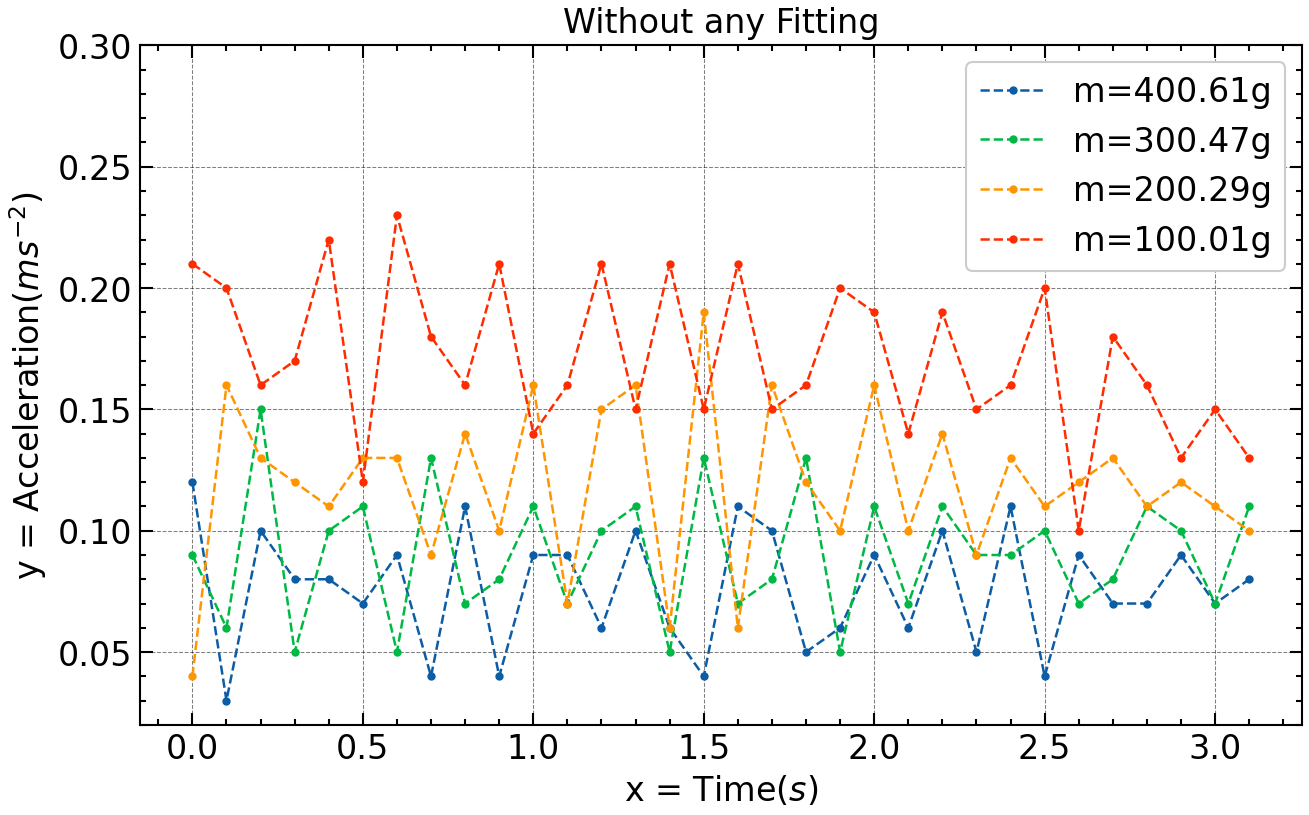
\includegraphics[scale=0.7]{acc vs time (no-fit).png}
	\caption{Acceleration vs. Time}
	\label{figure:accl2}%labeling the image
\end{figure}

The python code used to generate this plot is as follows:

\begin{lstlisting}
	import matplotlib.pyplot as plt
	import numpy as np
	plt.style.use(['science', 'notebook', 'grid'])
	from scipy.optimize import curve_fit
	
	plt.figure(figsize=(10,6), dpi=150)
	
	time, velo = np.genfromtxt('acceleration1.csv',  dtype = 'float', delimiter = ',', unpack = True, usecols=[0,1])
	plt.plot(time, velo, 'o--',lw=1.2, ms=3, label='m=400.61g')
	
	
	time, velo = np.genfromtxt('acceleration1.csv',  dtype = 'float', delimiter = ',', unpack = True, usecols=[0,2])
	plt.plot(time, velo, 'o--',lw=1.2, ms=3, label='m=300.47g')
	
	
	time, velo = np.genfromtxt('acceleration1.csv',  dtype = 'float', delimiter = ',', unpack = True, usecols=[0,3])
	plt.plot(time, velo, 'o--',lw=1.2, ms=3, label='m=200.29g')
	
	
	time, velo = np.genfromtxt('acceleration1.csv',  dtype = 'float', delimiter = ',', unpack = True, usecols=[0,4])
	plt.plot(time, velo, 'o--',lw=1.2, ms=3, label='m=100.01g')
	plt.ylim(top=0.3)
	plt.title('Without any Fitting')
	plt.xlabel('x = Time($s$)')
	plt.ylabel(r'y = Acceleration($ms^{-2}$)')
	plt.legend()
	plt.savefig('acc vs time (no-fit).png')
	plt.show()
\end{lstlisting}

\pagebreak

\textbf{Mass vs. Inverse Fitted Acceleration Graph:-}
 	
 	\begin{figure}[H]
 		\centering
 		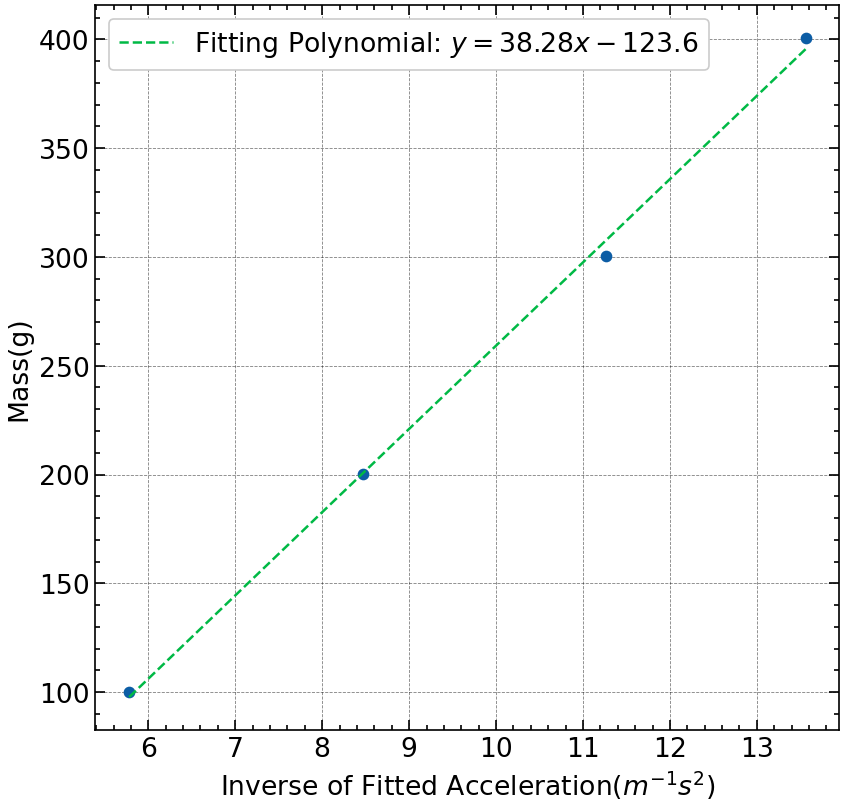
\includegraphics[scale=0.8]{final2.png}
 		\caption{Mass vs. Inverse of Acceleration}
 		\label{figure:nick}%labeling the image
 	\end{figure}
 
 Python code used for plotting and fitting is as follows:
 
 \begin{lstlisting}
 	import matplotlib.pyplot as plt
 	import numpy as np
 	plt.style.use(['science', 'notebook', 'grid'])
 	from scipy.optimize import curve_fit
 	
 	force = [100.01, 200.29, 300.47, 400.61]
 	inaccln = [5.78, 8.47, 11.26, 13.56]
 	plt.figure(figsize=(8,8), dpi=120)
 	plt.plot(inaccln, force, 'o')
 	z, res, _, sing, _ = np.polyfit(inaccln, force, 1, full='True')
 	f = np.poly1d(z)
 	print ("Fitting polynomial =",f)
 	print ('Sum of Residual Values =',res)
 	print('Singluar Asymptotic Errors =',sing)
 	inaccln_opt = np.linspace(inaccln[0], inaccln[-1], 500)
 	force_opt = f(inaccln_opt)
 	plt.xlabel ('Inverse of Fitted Acceleration($ms^{-2}$)')
 	plt.ylabel ('Force (= mg)')
 	plt.plot(inaccln_opt, force_opt, '--', lw=1.5, label=r'Fitting Polynomial: $y = 38.28x - 123.6$')
 	plt.legend()
 	plt.savefig('final2.png')
 	plt.show()
 \end{lstlisting}

\subsection{Error Analysis for Fixed Force Case:}

The sum of residual values generated by the above code is:
$$\texttt{Sum\ of\ Residual\ Values} = 80.46831428$$
And the asymptotic errors in each of the parameters of the fitting polynomial is:
\begin{table}[!ht]
	\centering
	\begin{tabular}{|l|l|}
		\hline
		Parameters & Singular Asymptotic Error \\ \hline
		a (or F) & 1.39928567 \\ \hline
		b & 0.20493804 \\ \hline
	\end{tabular}
	\caption{Errors in parameters of Fitting Polynomial}
	\label{error}
\end{table}

Accepted Value of  Force $= 0.0405N$\\
Value of Force obtained from the above graph fitting(i.e., slope of m vs. $a^{-1}$ graph) $= 0.03828N$\\
Absolute Error in Force $= |0.0405N - 0.03828N| = 0.00222N$\\
Relative Percentage Error $= \dfrac{0.0022}{0.0405} \times 100\% = 5.4321\%$

\pagebreak

\section{Conclusion}

We have verified using experimental data (empirically), that:
\begin{enumerate}
	\item Force is directly proportional to acceleration.
	\item Mass is inversely proportional to acceleration with slope of the graph representing Force.
\end{enumerate}

Thus, we have experimentally proven Newton's $2^{nd}$ Law of Motion.

\section{Acknowledgement}
I would like to express my gratitude to:
\begin{enumerate}
	\item Prof. Ritesh Kumar Singh for allowing us to write this lab report and providing us the data for the experiment.
	\item The creators of the NumPy, SciPy, csv, and MatPlotlib python packages which helped me plot the graphs and perform fitting on the provided data.
\end{enumerate}
\end{document}